%% LyX 2.2.2 created this file.  For more info, see http://www.lyx.org/.
%% Do not edit unless you really know what you are doing.
\documentclass[english]{article}
\usepackage[T1]{fontenc}
\usepackage[latin9]{inputenc}
\usepackage{amsbsy}
\usepackage[section]{placeins}
\usepackage{amssymb}
\usepackage{amsmath}
\usepackage{graphicx}
\usepackage{babel}
\usepackage{color}
\usepackage{natbib}
\usepackage{grffile}

\newcommand{\rdh}[2]{\textcolor{blue}{#1 {\em (RDH: #2)}}}

\title{CS5340: Project Report}
\author{\begin{tabular}{rl}
  \textbf{Professor:} & Lee Gim Hee \\
  \textbf{Working Group:} & Rahul Soni (A0174414J) \\ & Kyaw Zaw Lin (A0024997N)
\end{tabular}}


\begin{document}
\maketitle

\begin{abstract}
\textit{In this report, we summarize our approaches on (i) denoising using Gibbs sampling and (ii) segmentation using Gaussian Mixture Model.\\
For Denoising, we use Gibbs sampling on Ising CRF model with Gaussian observation model. It works well and we are able to obtain 99.84\% accuracy on the given image with no noise. 
In Segmentation, we implement GMM using various numerically stable techniques for computation for example log of determinant of Covariance matrix to avoid underflow/overflow. \textbf{We observed that the Maximum likelihood based parameter estimation does not work very well for the image "zebra.jpg". Hence we implemented MAP based update rule which gives impressive performance upgrade on the particular example}}

\begin{equation}\label{eq1}
    p(\theta | \mathbf{x}) = p(\mathbf{x} | \theta)p(\theta)
\end{equation}

The conjugate prior, $p(\theta)$ was challenging, especially to formulate it for a multi-variate distribution and derive the update rule for mean and covariance matrix. We also run over training models multiple times to find a right combination of hyperparameters: $\alpha$, $\gamma$, $\delta$, $\Psi$. We highlight results from both MLE and MAP in some examples. 

\end{abstract}

\pagebreak

\section{Question 1}

Gibbs sampling is one of the MCMC algorithms. Given a set of random variables, $\{z_i:i=1,...,M\}$, and  time steps $\tau=1,...T$,
\begin{itemize}
	\item $z_1^{\{\tau+1\}} \sim  p(z_1|z_2^{\{\tau\}},...,z_M^{\{\tau\}})$
	\item $z_2^{\{\tau+1\}} \sim  p(z_2|z_2^{\{\tau+1\}},...,z_M^{\{\tau\}})$
	\item $...$
	\item $z_M^{\{\tau+1\}} \sim  p(z_M|z_2^{\{\tau+1\}},...,z_{M-1}^{\{\tau+1\}})$
\end{itemize}

In other words, at each time step, we sample from the full conditional of one variable, also written $p(z_i|z_{-i})$, which is the probability of $z_i$ given all others. Then we update the state of variable and proceed until time step $T$. The initial samples are discarded until the Markov chain has burned in, or entered its stationary distribution. In our implementation, we discard initial 25\% of the samples. 

When applying Gibbs sampling image denoising problem, we use the pairwise Ising CRF prior where pairwise potentials $\psi_{st}(x_s,x_t)$ are given by $exp(Jx_sx_t)$ and $ x_s,x_t \in \{-1,+1\}$. Note that to infer $p(x_i)$, we only need to know the Markov blanket of $i$ which are the neighbours of $i$.


\begin{align} 
\begin{split}
p(x_t|x_{-t},\theta) & \propto \prod_{s\in nbr(t)} \psi_{st}(x_s,x_t)\\
%					 & \propto \prod_{s\in nbr(t)} exp(Jx_sx_t)\\
\end{split}					
\end{align} 

The model can be further extended by incorporating local evidence $\psi_t(x_t)$. 

\begin{align} 
\begin{split}
	p(x_t|x_{-t},y,\theta) & \propto \psi_t(x_t) \prod_{s\in nbr(t)} \psi_{st}(x_s,x_t)\\
%	& \propto \prod_{s\in nbr(t)} exp(Jx_sx_t)\\
\end{split}						
\end{align} 

By using Gaussian observation model where $\psi_t(x_t) = \mathcal{N}(y_t|x_t,\sigma^2)$, and normalizing we obtain the probability of a particular pixel being +1:


\begin{align} 
\begin{split}
&p(x_t=+1|x_{-t},y,\theta) \\
&    = \dfrac{\psi_t(+1) \prod_{s\in nbr(t)} \psi_{st}(x_t=+1,x_s)}{\psi_t(+1) \prod_{s\in nbr(t)} \psi_{st}(x_t=+1,x_s) + \psi_t(-1)\prod_{s\in nbr(t)} \psi_{st}(x_t=-1,x_s)}\\
&    = \dfrac{\psi_t(+1) exp[J\sum_{s\in nbr(t)}{x_s}]}{\psi_t(+1) exp[J\sum_{s\in nbr(t)}{x_s}]+\psi_t(-1) exp[-J\sum_{s\in nbr(t)}{x_s}]}\\
\end{split}						
\end{align} 


We then set $p(x_t)$ to $+1$ with this probability and otherwise setting it to $-1$ and let the sampling run for time $T$ and return the mean of samples as final estimate.

\subsection{Implementation Details and results}
Note that for local evidence term, there is a need to guess the value of $\sigma$. If underestimate noise level, we have reduced noise reduction. If we overestimate noise level, then our original signal maybe corrupted. Since we have one original image, we use it to check the accuracy of restoration and to estimate $\sigma$. We used $\sigma=1$ with approximately 99.84\% accuracy in recovered signal.

\begin{figure}[!htb]
\minipage{0.25\textwidth}
  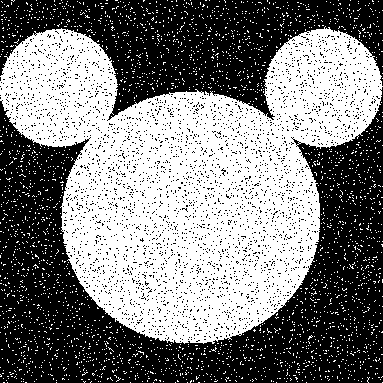
\includegraphics[width=\linewidth]{a1_sigma_levels/0.5.png}
\endminipage\hfill
\minipage{0.25\textwidth}
  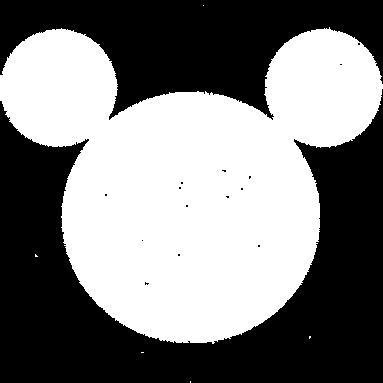
\includegraphics[width=\linewidth]{a1_sigma_levels/0.7.png}
\endminipage\hfill
\minipage{0.25\textwidth}%
  
\includegraphics[width=\linewidth]{a1_sigma_levels/1.0.png}
\endminipage
\minipage{0.25\textwidth}%
  
\includegraphics[width=\linewidth]{a1_sigma_levels/6.0.png}
\endminipage
\caption{Denoised results with sigma [0.5,0.7,\textbf{1.0},6.0], from left to right. As we can see with large $\sigma$, the shape of the circle starts to deform and with small $\sigma$, there is not enough reduction in noise.Highlighted in bold is the optimal $\sigma$}\label{fig:a1_sigma_levels}.
\end{figure}
As an implementation trick, we used convolution with $ k = \bigl( \begin{smallmatrix}0 & 1 & 0\\ 1 & 0 & 1\\ 0 & 1 & 0\end{smallmatrix}\bigr)$ to evaluate the term $\sum_{s\in nbr(t)}{x_s}$. This significantly speeds up run time performance.
\begin{figure}[!htb]
\minipage{0.25\textwidth}
  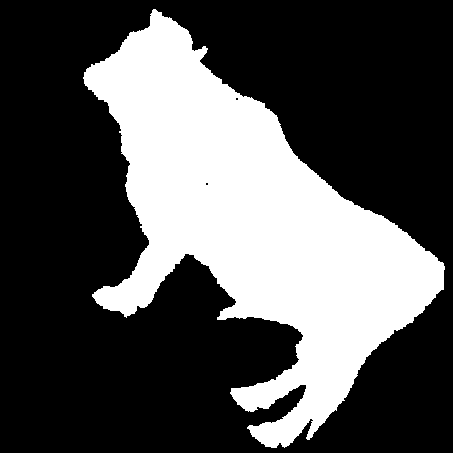
\includegraphics[width=\linewidth]{a1_results/1_noise.png}
\endminipage\hfill
\minipage{0.25\textwidth}
  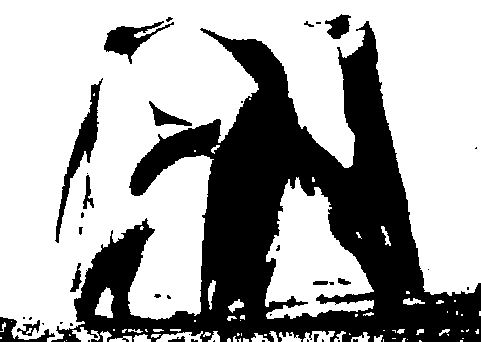
\includegraphics[width=\linewidth]{a1_results/2_noise.png}
\endminipage\hfill
\minipage{0.25\textwidth}%
  
\includegraphics[width=\linewidth]{a1_results/3_noise.png}
\endminipage
\minipage{0.25\textwidth}%
  
\includegraphics[width=\linewidth]{a1_results/4_noise.png}
\endminipage
\caption{Final results. We run with $\sigma=1$, burn-in=5, total samples=15 and $J=1$}\label{fig:a1_results}.
\end{figure}

\pagebreak

\section{Question 2}
\subsection{Experiment Setup}
We implement both MLE and MAP based  parameter update for GMM. To initialize the parameters of the multi-variate Gaussian distribution, we use the K-means clustering (using SciKit-Learn library) which in turn is augmented with randomized seeding technique \cite{arthur2007k} \textit{k-means++}. From numerical stability perspective, we calculate log of Determinant of Covariance matrix and parameters of Conjugate distribution which helps avoid overflow/underflow errors. \\

\underline{\textbf{Normalization}}: We experiment with both $l_2$ normalizing the input along the channel dim (normalize each $R^3$ input vector)  and $l_2$ normalizing along the feature dimension (normalize all the three R,G,B frames independently). Following bench-marking results on "cow.jpg" image using $l_2$ along the channel and features illustrate the difference:
\begin{figure}[!htb]
\minipage{0.25\textwidth}
  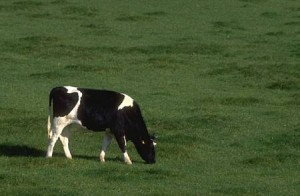
\includegraphics[width=\linewidth]{images/cow.jpg}
\endminipage\hfill
\minipage{0.25\textwidth}
  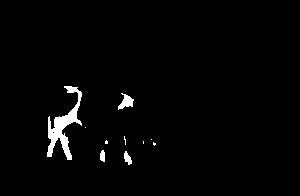
\includegraphics[width=\linewidth]{images/feat_l2_cow_copy_mask.jpg}
\endminipage\hfill
\minipage{0.25\textwidth}%
  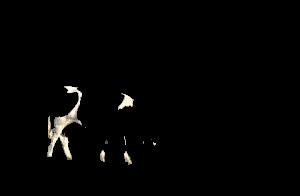
\includegraphics[width=\linewidth]{images/feat_l2_cow_copy_seg1.jpg}
\endminipage
\minipage{0.25\textwidth}%
  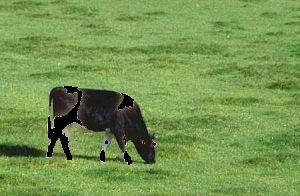
\includegraphics[width=\linewidth]{images/feat_l2_cow_copy_seg2.jpg}
\endminipage
\caption{Segmentation using \underline{$l_2$ norm along the feature axis}: Each frame/channel of the image is normalized using $l_2$ norm of all pixel values on that feature frame. We see that in the background segmentation, \textbf{more than 50\% of the foreground (in this case cow) is appearing in the background} as well}\label{fig:a2_cow}
\end{figure}

\begin{figure}[!htb]
\minipage{0.25\textwidth}
  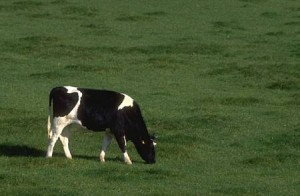
\includegraphics[width=\linewidth]{images/cow.jpg}
\endminipage\hfill
\minipage{0.25\textwidth}
  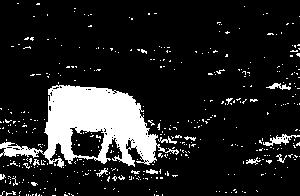
\includegraphics[width=\linewidth]{images/channel_l2_cow_copy_mask.jpg}
\endminipage\hfill
\minipage{0.25\textwidth}%
  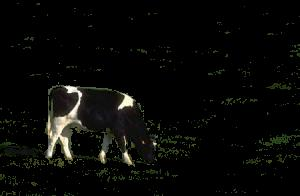
\includegraphics[width=\linewidth]{images/channel_l2_cow_copy_seg1.jpg}
\endminipage
\minipage{0.25\textwidth}%
  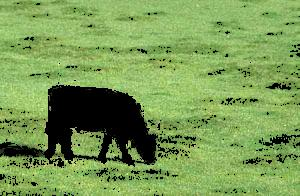
\includegraphics[width=\linewidth]{images/channel_l2_cow_copy_seg2.jpg}
\endminipage
\caption{Segmentation using \underline{$l_2$ norm along the channel axis}: Each data point ($\in R^3$) of the image is normalized using $l_2$ norm of all the three pixel values.}\label{fig:a2_cow}.
\end{figure}

{$l_2$ norm along each feature frames also \textbf{fails for the image "zebra.jpg" under MLE estimate} (similar to "cow.jpg" example above). The results are as expected because the \textbf{$l_2$ along each feature frames mixes the features values for different objects in the image (in our case foreground and background), hence the loss of information}. \\

However, feature-wise normalization can be useful in some extreme cases. For example in image "zebra.jpg", we see that the feature normalization failed under MLE estimate, but the features in zebra are correlated with the background (due to black strips). So the feature wise normalization for "zebra.jpg" should work but with an estimator stronger than MLE. Hence, using a MAP estimator, we see impressive improvement in "zebra.jpg" using the feature normalization (more details in MAP section). So \textbf{"zebra.jpg" is a special case}. For rest of the images, we continue to use the $l_2$ norm along each input vector $\in R^3$

\subsection{Maximum Likelihood Estimation (MLE)}
Here are the results of GMM using the maximum likelihood update rule (we do not show the iterative update rule equations which is trivial. We will, however, mention the multi-variate conjugate prior formulation for MAP in the next section)

\begin{figure}[!htb]
\minipage{0.25\textwidth}
  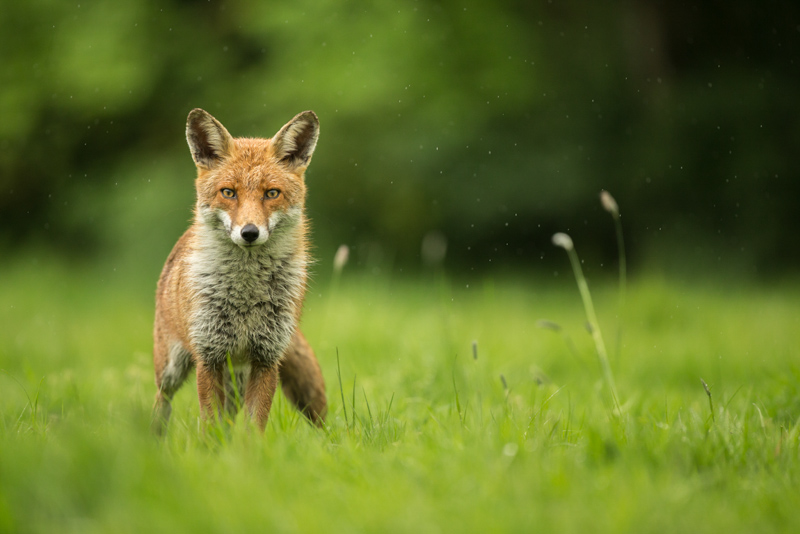
\includegraphics[width=\linewidth]{images/fox.jpg}
\endminipage\hfill
\minipage{0.25\textwidth}
  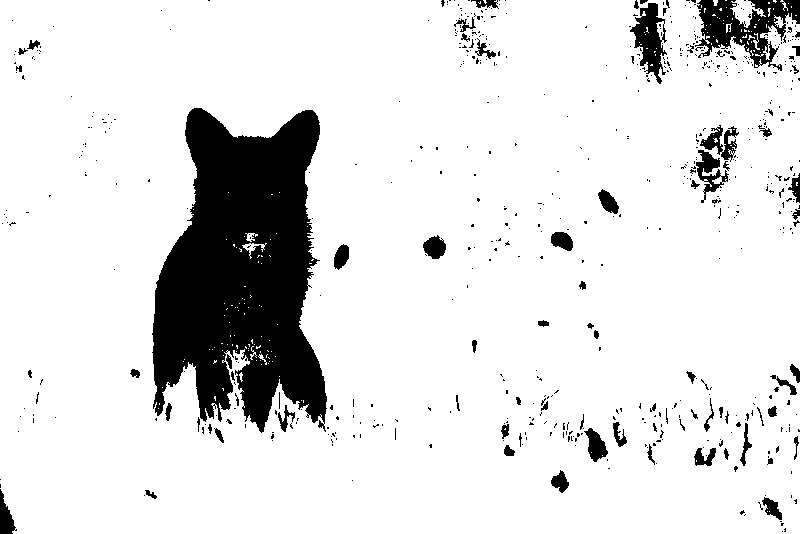
\includegraphics[width=\linewidth]{images/fox_mask.jpg}
\endminipage\hfill
\minipage{0.25\textwidth}%
  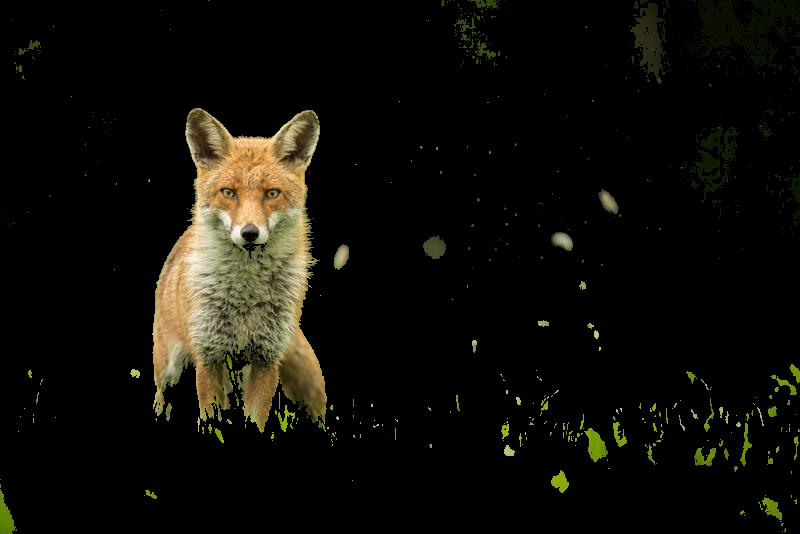
\includegraphics[width=\linewidth]{images/fox_seg2.jpg}
\endminipage
\minipage{0.25\textwidth}%
  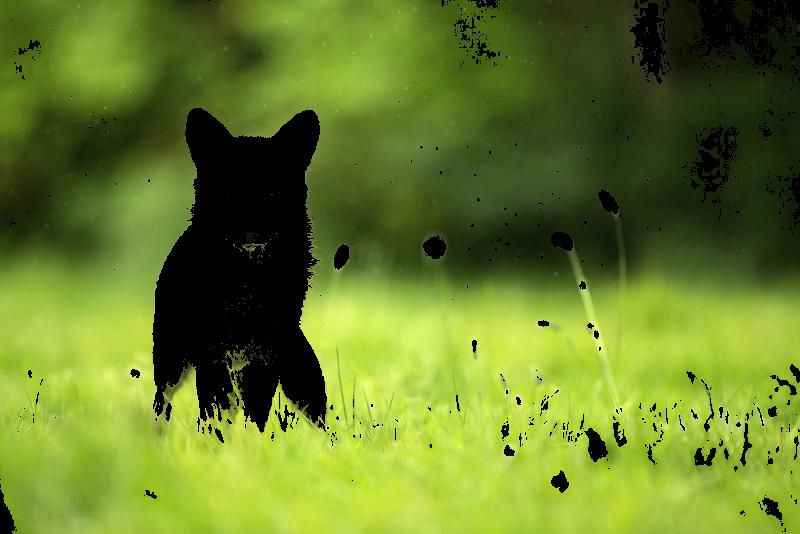
\includegraphics[width=\linewidth]{images/fox_seg1.jpg}
\endminipage
\caption{Foreground/background segmentation using MLE estimation and $l_2$ norm along each data point (observation of the random vector $\in R^3$)}\label{fig:a2_cow}.
\end{figure}

\begin{figure}[!htb]
\minipage{0.25\textwidth}
  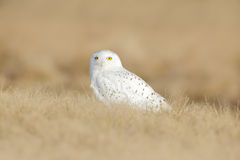
\includegraphics[width=\linewidth]{images/owl.jpg}
\endminipage\hfill
\minipage{0.25\textwidth}
  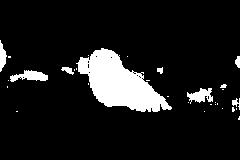
\includegraphics[width=\linewidth]{images/owl_mask.jpg}
\endminipage\hfill
\minipage{0.25\textwidth}%
  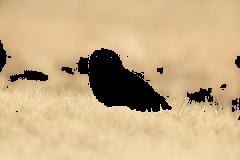
\includegraphics[width=\linewidth]{images/owl_seg2.jpg}
\endminipage
\minipage{0.25\textwidth}%
  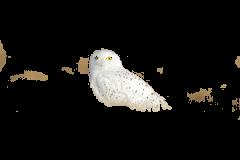
\includegraphics[width=\linewidth]{images/owl_seg1.jpg}
\endminipage
\caption{Foreground/background segmentation using MLE estimation and $l_2$ norm along each data point (observation of the random vector $\in R^3$)}\label{fig:a2_cow}.
\end{figure}

\begin{figure}[!htb]
\minipage{0.25\textwidth}
  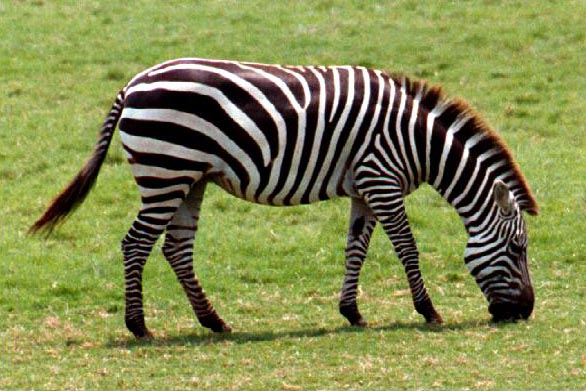
\includegraphics[width=\linewidth]{images/zebra.jpg}
\endminipage\hfill
\minipage{0.25\textwidth}
  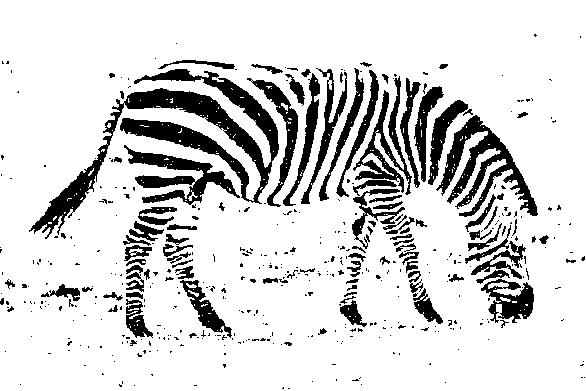
\includegraphics[width=\linewidth]{images/zebra_mask.jpg}
\endminipage\hfill
\minipage{0.25\textwidth}%
  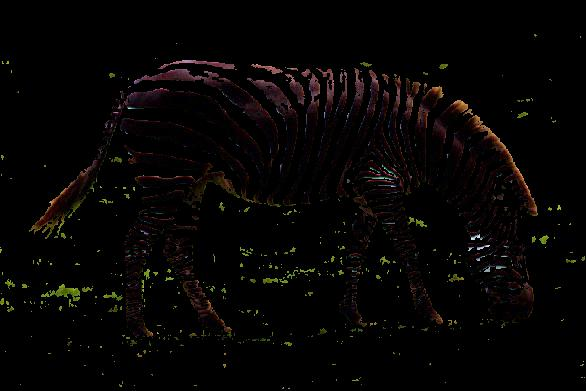
\includegraphics[width=\linewidth]{images/zebra_seg2.jpg}
\endminipage
\minipage{0.25\textwidth}%
  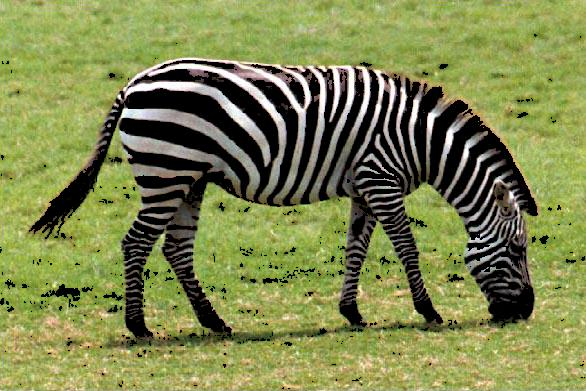
\includegraphics[width=\linewidth]{images/zebra_seg1.jpg}
\endminipage
\caption{Foreground/background segmentation using MLE estimation and $l_2$ norm along each data point (observation of the random vector $\in R^3$)}\label{fig:a2_cow}.
\end{figure}


\subsection{MAP Estimator}
MAP estimation is given by maximizing the following conditional distribution:
\begin{equation}\label{eq1}
    p(\theta | \mathbf{x}) = p(\mathbf{x} | \theta)p(\theta)
\end{equation}

Here the distribution, $p(\theta)$ of the parameters of the Multi-variate Gaussian distribution is given by the Normal-Inverse-Gamma distribution. From the lecture notes, we use the definition on multi-variate distribution (slide 59, lecture 1) and formulate the update rule for parameters (mean and variance) under the influence of this conjugate prior. We also simply $p(\theta)$ by evaluating the $log(p(\theta))$ and remove constants ($K$) that do not affect the maximization criteria. Here is the conjugate prior distribution and corresponding parameter update rule:

\begin{equation}\label{eq11}
    \begin{split}
     log(p(\theta)) &= \frac{K * exp \bigg(-\frac{1}{2} Tr\big(\pmb{\Psi\Sigma}^{-1}\big) + \gamma\big(\pmb{\mu} - \pmb{\delta} \big)^T\pmb{\Sigma}^{-1}\big(\pmb{\mu} - \pmb{\delta} \big) \bigg)}{K * |\pmb{\Sigma}|^{\alpha + d + 2}} \\ \\
     \pmb{\hat{\mu}} & \longleftarrow \frac{\sum_{i=1}^{N}\Big(\pmb{x_i}\Big) + \gamma\pmb{\delta}}{N + \gamma} \\ \\
     \pmb{\hat{\Sigma}} & \longleftarrow \frac{\sum_{i=1}^{N}\Big(\pmb{x_i} - \pmb{\mu}\Big)\Big(\pmb{x_i} - \pmb{\mu}\Big)^T + \gamma\Big(\pmb{\mu} - \pmb{\delta}\Big)\Big(\pmb{\mu} - \pmb{\delta}\Big)^T + 2\pmb{\Psi}}{N + 3 + 2\alpha}
    \end{split}
\end{equation}

We modify the EM algorithm and update the parameters $\pmb{\mu}$, and $\pmb{\Sigma}$ according to equation[6]. During the inference phase, (maximization step), we use equation[5], i.e., we multiple the MLE probability with the conjugate prior given in equation[6]. As we can see in the results below, we observe significant change in the image "zebra.jpg". \textbf{Hence, by adding the conjugate prior distribution, we overcome the limitation of MLE estimate}}.
\begin{figure}[!htb]
\minipage{0.25\textwidth}
  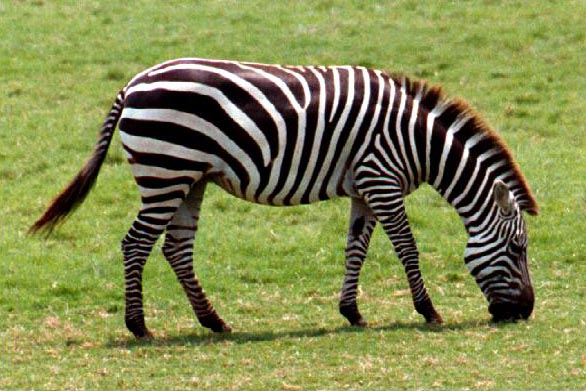
\includegraphics[width=\linewidth]{images/zebra.jpg}
\endminipage\hfill
\minipage{0.25\textwidth}
  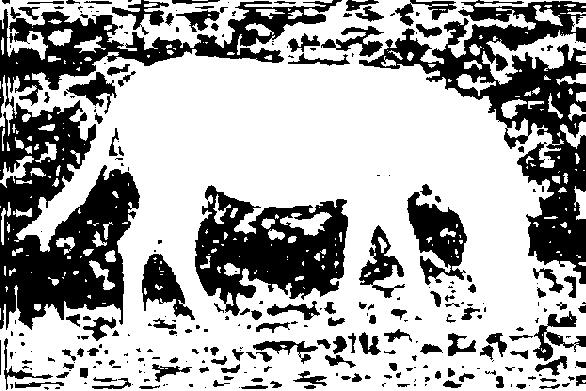
\includegraphics[width=\linewidth]{images/map_zebra_mask.jpg}
\endminipage\hfill
\minipage{0.25\textwidth}%
  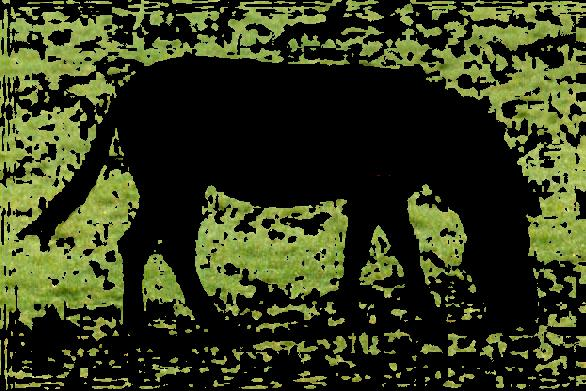
\includegraphics[width=\linewidth]{images/map_zebra_seg2.jpg}
\endminipage
\minipage{0.25\textwidth}%
  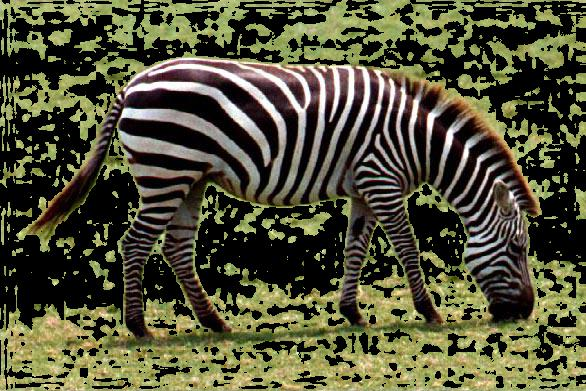
\includegraphics[width=\linewidth]{images/map_zebra_seg1.jpg}
\endminipage
\caption{Foreground/background segmentation using MAP estimation and $l_2$ norm along each feature frames. \textbf{This is the only special data point where  feature normalization works better than channel normalization}. Compared to fig[7] above, we observe significant improvement using MAP}\label{fig:a2_cow}.
\end{figure}

\subsection{Code Running Instructions:}
\subsubsection{Question 1}
No special instructions are required for running code for this question. Executing the following inside the "a1" folder is enough.

\begin{verbatim}
python denoise.py
\end{verbatim}
The software requirements are similar to those for Question 2.

\subsubsection{Question 2}
Run the script "gmm.py" with following arguments:
\begin{verbatim}
    estimator (str): One of "mle" or "map". If this argument is not passed,
                "mle" is implemented by default
    num_iter (int): Default value of 50
    image_name (str): image to segment ("cow.jpg", "fox.jpg", "zebra.jpg")
\end{verbatim}

The script expects a folder named "a2" inside the "project" folder workspace. Since scripts builds paths relative to where it is run from, please run the script from the directory it is present (project in this case). Here is the sample run command:
\begin{verbatim}
python gmm.py --estimator map --num_iter 50 --image_name zebra.jpg
\end{verbatim}

Additionally, the code has dependency on following libraries:
\begin{verbatim}
python (2.7.14)
PIL (1.1.7)
scikit-learn (0.19.1)
tqdm (4.19.4)
numpy (1.13.3)
\end{verbatim}


\bibliographystyle{plain}
\bibliography{ml_17}

\end{document}
